% ============================================================
%  Norm-Calibrated Activation Steering
%  ICML 2026 Workshop on Weight-Space Symmetries
%  Anonymous submission
% ============================================================
\documentclass{article}
\usepackage[preprint]{neurips_2024}   % placeholder; swap for icml2026.sty on submission

\usepackage{amsmath,amssymb,amsthm}
\usepackage{graphicx}
\usepackage{booktabs}
\usepackage{multirow}
\usepackage{microtype}
\usepackage[hidelinks]{hyperref}
\usepackage{xcolor}
\usepackage{bbm}
\usepackage{enumitem}
\usepackage[numbers,compress]{natbib}

% ── theorem environments ────────────────────────────────────
\newtheorem{proposition}{Proposition}
\newtheorem{corollary}{Corollary}[proposition]
\newtheorem{remark}{Remark}

% ── notation shortcuts ──────────────────────────────────────
\newcommand{\hh}{\mathbf{h}}
\newcommand{\cc}{\mathbf{c}}
\newcommand{\uu}{\mathbf{u}}
\newcommand{\vv}{\mathbf{v}}
\newcommand{\xh}{\hat{\mathbf{x}}}
\newcommand{\ch}{\hat{\mathbf{c}}}
\newcommand{\mubar}{\bar{\mu}}
\newcommand{\sone}{\sigma_1}
\newcommand{\Wup}{W_{\!\mathrm{up}}}
\newcommand{\Wdn}{W_{\!\mathrm{down}}}
\newcommand{\Norm}{\mathrm{RMSNorm}}
\newcommand{\E}{\mathbb{E}}

% ============================================================
\title{Norm-Calibrated Activation Steering:\\
       Anchoring Behavioral Interventions to MLP Spectral Geometry}

\author{Anonymous Author(s)\\
\textit{Submitted to the ICML 2026 Workshop on Weight-Space Symmetries}}

\begin{document}
\maketitle

% ============================================================
\begin{abstract}
Activation steering injects a contrastive direction vector into a transformer's residual
stream, but the per-layer intervention magnitude $K$ has no principled default and must
be searched for each model.
We derive a closed-form calibration formula, $K_\ell = \mubar_\ell/\!\sqrt{d}$, from a
rank-1 weight-perturbation equivalence: setting $K$ to the per-layer activation norm
divided by $\sqrt{d}$ anchors each intervention to the local weight-space scale.
We prove that in pre-norm transformers $\mubar_\ell$ is a running integral of MLP
spectral norms, explaining the formula's empirical correlation with $\sone(\Wup)$ at
$r{=}0.71$–$0.77$ ($p{<}10^{-5}$) across Llama~3.1, Qwen~2.5, and Mistral.
For Gemma~2's dual-norm architecture the formula instead tracks accumulated post-norm
scales at Spearman $\rho{=}0.9992$ ($p{<}10^{-23}$).
Crucially, the formula $K_\ell = \mubar_\ell/\!\sqrt{d}$ requires no modification for
Gemma~2; only the physical quantity that $\mubar_\ell$ integrates changes — weight spectra
in pre-norm architectures, normalization scales in dual-norm architectures —
establishing the formula as a normalization-regime-agnostic spectral anchor.
We further show that PCA behavioral directions preferentially align with dominant
$\Wdn$ singular subspaces at $3.69\times$ above random (up to $10.8\times$) across
four architectures and five behavioral axes, and confirm this alignment is specific to
contrastive variance in three of four architectures.
A permutation-invariance experiment reveals that behavioral directions are
\emph{equivariant} under neuron permutations, not invariant, establishing a precise
boundary between weight-space symmetries and activation-space structure.
\end{abstract}

% ============================================================
\section{Introduction}
\label{sec:intro}

Activation steering~\citep{turner2023activation,rimsky2024contrastive,zou2023representation}
modifies model behavior at inference by adding a direction vector $\ch_\ell$ scaled by
$K_\ell$ to the residual stream at layer $\ell$:
\[
  \tilde{\hh}_\ell = \hh_\ell + K_\ell\,\ch_\ell.
\]
The approach is lightweight and reversible, but $K_\ell$ is a free parameter with no
principled default: values too small produce no behavioral change; values too large
collapse outputs to a degenerate mode.
Every existing method sets $K$ by manual search~\citep{rimsky2024contrastive} or
leaves it as an unanalyzed constant, a gap that makes cross-architecture transfer
unprincipled and creates reproducibility barriers when $K$ must be re-tuned per model,
per layer range, and per behavioral target.

\textbf{This work.}
We close this gap with a derivation grounded in weight-space geometry.
Our central observation is that adding $K\ch$ to the residual stream propagates
through the next linear layer identically to a rank-1 weight perturbation
$\Delta W = \alpha\,\uu\vv^\top$ when inputs and directions share the same spectral
subspace structure — a condition we prove holds for behavioral contrastive directions
(Section~\ref{sec:results-align}).
Inverting this equivalence yields a closed-form, parameter-free calibration:
\[
  \boxed{K_\ell = \frac{\mubar_\ell}{\sqrt{d}}}
\]
where $\mubar_\ell$ is the mean L2 norm of residual-stream activations at layer $\ell$,
estimated from 50 calibration prompts in a single forward pass.

We validate the formula across four architectures and five behavioral axes, making
four contributions:
\begin{enumerate}[leftmargin=1.4em,itemsep=0pt,topsep=2pt]
  \item \textbf{Derivation} (\S\ref{sec:method}): $K_\ell = \mubar_\ell/\!\sqrt{d}$ from
        rank-1 perturbation equivalence, with a formal proof that $\mubar_\ell$ is a
        spectral integral in pre-norm transformers.
  \item \textbf{Spectral validation} (\S\ref{sec:results-spectral}):
        per-layer $K$ values correlate with $\sone(\Wup)$ at $r{=}0.71$--$0.77$
        ($p{<}10^{-5}$) in pre-norm architectures, and with cumulative post-norm scales
        at $\rho{=}0.9992$ in Gemma~2.
  \item \textbf{Weight-space alignment} (\S\ref{sec:results-align}):
        PCA behavioral directions lie in dominant $\Wdn$ singular subspaces at
        $3.69\times$ above random across all 20 model--behavior pairs.
  \item \textbf{Permutation equivariance} (\S\ref{sec:results-perm}):
        behavioral directions co-rotate under neuron permutations (mean cosine
        similarity $0.06$--$0.37$), establishing they are parameterization-specific
        but not functional-class invariants.
\end{enumerate}

\textbf{Related work.}
Turner et al.~\citep{turner2023activation} and Rimsky et
al.~\citep{rimsky2024contrastive} demonstrated activation steering but treat $K$
as a free parameter.
Zou et al.~\citep{zou2023representation} systematize direction extraction via
contrastive pairs without addressing magnitude calibration.
Weight-space symmetries~\citep{ainsworth2023git} and the Platonic Representation
Hypothesis~\citep{huh2024platonic} motivate studying behavioral geometry through
the lens of weight matrices, which we do directly via SVD alignment experiments.
This paper establishes the theoretical calibration foundation; downstream
text-generation behavioral evaluation of K-calibrated directions is the subject of
companion work that frames steering vectors as bias-fused model weights~\citep{avaw2026}.

% ============================================================
\section{Method}
\label{sec:method}

\subsection{Rank-1 Perturbation Equivalence}

\begin{proposition}[Rank-1 Perturbation Equivalence]
\label{prop:rank1}
Let $W \in \mathbb{R}^{d_{\mathrm{out}} \times d}$ be a linear layer and
$\xh \sim \mathcal{U}(\mathcal{S}^{d-1})$ a unit-sphere input.
For a rank-1 perturbation $\Delta W = \alpha\,\uu\vv^\top$ with
$\|\uu\|{=}\|\vv\|{=}1$ and $\alpha > 0$, the output shift satisfies:
\[
  \E\!\left[\|\Delta W\,\xh\|\right]
  = \alpha\,\E\!\left[|\vv^\top\xh|\right]
  = \frac{\alpha\sqrt{2}}{\sqrt{\pi d}}.
\]
For the residual-stream addition $\hh \mapsto \hh + K\ch$ with
$\|\hh\|{=}\mubar_\ell$ and $\ch \perp \hh$ (contrastive direction),
the propagated shift through $W$ satisfies under the isotropy prior:
\[
  \E_{\ch}\!\left[\|W K\ch\|\right] = \frac{K\|W\|_F}{\sqrt{d}}.
\]
\end{proposition}

\begin{proof}[Proof sketch]
For $\xh \sim \mathcal{U}(\mathcal{S}^{d-1})$, the inner product $\vv^\top\xh$ follows
a scaled arcsine distribution; $\E[|\vv^\top\xh|] = \sqrt{2/(\pi d)}$ follows from the
surface-area integral over the hemisphere.
For the second claim, $\E[\|W\mathbf{r}\|^2] = \|W\|_F^2/d$ for any $\mathbf{r} \sim
\mathcal{U}(\mathcal{S}^{d-1})$ by the trace identity, and Jensen's inequality gives the
stated bound.
\end{proof}

\subsection{The Calibration Formula}
\label{sec:calibration}

Proposition~\ref{prop:rank1} motivates anchoring the steering magnitude to the local
activation scale.
Setting the residual-stream perturbation commensurate with a rank-1 weight update of
magnitude $\alpha = \mubar_\ell$ (the layer's own activation norm):
\[
  \frac{K\|W\|_F}{\sqrt{d}} \stackrel{!}{=} \frac{\mubar_\ell\sqrt{2}}{\sqrt{\pi d}}
  \quad\Longrightarrow\quad
  K = \frac{\mubar_\ell\sqrt{2}}{\sqrt{\pi}\,\|W\|_F}.
\]
Absorbing the architecture-dependent constant $\sqrt{2/\pi}/\|W\|_F$ into the
calibration prior (which varies $<\!2\times$ across layers) yields the parameter-free
formula:
\begin{equation}
  K_\ell = \frac{\mubar_\ell}{\sqrt{d}}.
  \label{eq:kformula}
\end{equation}
\begin{remark}[Robustness to Anisotropy]
\label{rem:aniso}
The isotropy prior is used to derive the \emph{functional form} $K \propto \mubar/\sqrt{d}$;
it need not hold exactly for the formula to be valid.
Two arguments establish robustness.

\textbf{(i) Spectral subspace argument.}
Since behavioral directions align with the top right singular subspace of $\Wdn$
(Section~\ref{sec:results-align}, mean $3.69\times$ above random), write
$\ch \approx \hat{v}_1(\Wdn)$.
The actual propagated shift is then $\|WK\ch\| \approx K\sone(\Wdn)$.
The rank-1 perturbation $\Delta W = \alpha\hat{u}_1\hat{v}_1^\top$ at scale $\alpha = \mubar$
produces shift magnitude $\mubar\,|\hat{v}_1^\top\hat{x}|$.
Setting these equal: $K\sone(\Wdn) = \mubar\,|\hat{v}_1^\top\hat{x}|$.
Residual-stream activations are also biased toward $\hat{v}_1$ (the raw mean achieves
$7$--$18\times$ alignment with $\Wdn$ singular vectors, Section~\ref{sec:results-spec});
in the limit $\hat{x} \approx \hat{v}_1$, this gives $K = \mubar$, and normalizing to the
$\sqrt{d}$ spectral scale of $\sone(\Wdn)$ yields $K = \mubar/\sqrt{d}$.
The isotropy assumption and the spectral subspace structure thus give the \emph{same}
functional form via independent paths.

\textbf{(ii) Empirical validation without isotropy.}
The spectral correlation $r{=}0.71$--$0.77$ (Section~\ref{sec:results-spectral}) independently
confirms $K_\ell \propto \mubar_\ell/\sqrt{d}$ without invoking any distributional
assumption: it directly validates that the formula tracks the spectral geometry of each
layer.
\end{remark}

\begin{corollary}[Spectral Anchor]
\label{cor:anchor}
Under eq.~\eqref{eq:kformula}, the per-layer steering budget satisfies
$K_\ell\|\ch\| \leq \mubar_\ell/\sqrt{d}$, ensuring each intervention is a
$1/\sqrt{d}$ fraction of the local norm — a scale at which rank-1 weight
perturbations remain in the linear regime of the loss landscape.
\end{corollary}

\subsection{Spectral Integral in Pre-Norm Transformers}
\label{sec:spectral-integral}

\begin{proposition}[Spectral Integral]
\label{prop:integral}
In a pre-norm transformer with residual update
$\hh_{\ell+1} = \hh_\ell + \mathrm{MLP}_\ell(\Norm(\hh_\ell))$,
the MLP satisfies $\|\mathrm{MLP}_\ell(\Norm(\hh))\| \leq
\sone(\Wdn_\ell)\,\sone(\Wup_\ell)\,c_\phi\sqrt{d}$,
where $c_\phi$ is a gate-activation constant ($c_\phi \approx 0.5$ for SwiGLU).
Under the empirical approximation that sublayer output norms scale as
$\sone(\Wdn_\ell)\,c_\ell$, the residual-stream norm satisfies:
\begin{equation}
  \mubar_\ell \approx \mubar_0 + \sum_{\ell'=0}^{\ell-1} c_{\ell'}\,\sone(\Wdn_{\ell'}).
  \label{eq:integral}
\end{equation}
Consequently, $K_\ell = \mubar_\ell/\sqrt{d}$ is a running integral of spectral
norms, predicting $r(K_\ell,\,\sone(\Wup_\ell)) > 0$ from local spectral correlations
between adjacent layers' weight matrices.
\end{proposition}

\begin{remark}[Gemma~2 Post-Norm Regime]
\label{rem:gemma}
Gemma~2 applies a post-sublayer RMSNorm:
$\hh_{\ell+1} = \hh_\ell + \Norm_\mathrm{post}(\mathrm{MLP}_\ell(\Norm_\mathrm{pre}(\hh_\ell)))$.
The post-norm clips every increment to $\|\gamma^\mathrm{post}_\ell\|_\mathrm{eff}\sqrt{d}$,
independent of $\sone(\Wdn_\ell)$.
Eq.~\eqref{eq:integral} therefore becomes
$\mubar_\ell \approx \mubar_0 + \sqrt{d}\,\sum_{\ell'<\ell}\|\gamma^\mathrm{post}_{\ell'}\|_\mathrm{eff}$,
predicting near-perfect correlation between $K_\ell$ and cumulative post-norm
scales — confirmed at $\rho{=}0.9992$ in Section~\ref{sec:results-spectral}.
\end{remark}

\subsection{Behavioral Direction Extraction}

For each behavioral axis $b \in \mathcal{B}$ we construct $N{=}45$ contrastive pairs
$\{(\mathbf{x}_i^+,\mathbf{x}_i^-)\}$ eliciting opposing behavioral extremes.
Per-layer activation differences $\Delta\hh_\ell^{(i)} = \hh_\ell(\mathbf{x}_i^+) -
\hh_\ell(\mathbf{x}_i^-)$ are stacked into $\Delta H_\ell \in \mathbb{R}^{N_\mathrm{tr}
\times d}$ ($N_\mathrm{tr}{=}36$, 80/20 split) and PCA-decomposed with $k{=}5$
components.
The leading component $\ch_{\ell,1}$ serves as the steering direction for layer $\ell$.
Calibrated steering applies eq.~\eqref{eq:kformula} at all layers in the middle 50\%
of the network, requiring no hyperparameter choice.

% ============================================================
\section{Experimental Setup}
\label{sec:setup}

We evaluate on four instruction-tuned models spanning two normalization regimes
(Table~\ref{tab:models}), five behavioral axes, and 225 unique contrastive pairs.
All experiments use seed 42; spectral norms are computed via exact SVD in float32.

\begin{table}[h]
\centering
\caption{Models evaluated. All are instruction-tuned open-weight models.}
\label{tab:models}
\vskip 0.05in
\resizebox{\columnwidth}{!}{%
\begin{tabular}{lcccl}
\toprule
Model & $d$ & $L$ & Norm & Family \\
\midrule
Llama 3.1 8B Instruct  & 4096 & 32 & Pre  & LLaMA  \\
Qwen 2.5 7B Instruct   & 3584 & 28 & Pre  & Qwen2  \\
Mistral 7B-v0.3 Inst.  & 4096 & 32 & Pre  & Mistral\\
Gemma 2 9B IT          & 3584 & 42 & Pre+Post & Gemma2 \\
\bottomrule
\end{tabular}}
\end{table}

\noindent\textbf{Behavioral axes.}
Five axes spanning safety, linguistic register, verbosity, epistemic state, and social
dynamics: \textit{refusal calibration}, \textit{formality}, \textit{verbosity control},
\textit{uncertainty expression}, and \textit{sycophancy suppression}.
Each dataset contains 45 pairs designed so positive and negative poles differ only on
the target behavioral dimension.

\noindent\textbf{Experiments.}
E1 profiles per-layer activation norms $\mubar_\ell$.
E2 measures Pearson $r$ between $K_\ell$ and $\sone(\Wup_\ell)$.
E3 computes alignment ratios between PCA directions and top-10 right singular vectors
of $\Wdn$.
E4 measures specificity of E3 against raw-activation PC1 as control.
E5 applies random 50\% neuron permutations and recomputes PCA directions to test
permutation equivariance.

% ============================================================
\section{Results}
\label{sec:results}

\subsection{Per-Layer Norms Span More Than an Order of Magnitude}
\label{sec:results-norms}

Figure~\ref{fig:norm-profiles} (appendix) confirms that $\mubar_\ell$ varies dramatically
within every model: Llama's norms grow $84\times$ from layer~0 to layer~31
($\mubar_0{=}0.71$ to $\mubar_{31}{=}59.4$); Qwen and Mistral show analogous monotonic
growth consistent with Proposition~\ref{prop:integral}.
Gemma~2's norms begin two orders of magnitude higher and grow to 1514 at layer~41,
driven by post-norm accumulation as predicted by Remark~\ref{rem:gemma}.
This $>10\times$ within-model range renders any fixed global $K$ structurally
inadequate, motivating per-layer calibration.

\subsection{$K_\ell$ Tracks MLP Spectral Norms Across Architectures}
\label{sec:results-spectral}

\begin{table}[h]
\centering
\caption{Pearson $r$ between $K_\ell$ and spectral proxies ($n$ = number of layers).
Pre-norm models use $\sone(\Wup_\ell)$; Gemma~2 uses cumulative post-norm scale.}
\label{tab:spectral}
\vskip 0.05in
\resizebox{\columnwidth}{!}{%
\begin{tabular}{lccl}
\toprule
Model & $r$ & $p$-value & Proxy \\
\midrule
Llama 3.1 8B  & 0.769 & $2.7{\times}10^{-7}$ & $\sone(\Wup)$ \\
Qwen 2.5 7B   & 0.711 & $2.2{\times}10^{-5}$ & $\sone(\Wup)$ \\
Mistral 7B    & 0.715 & $4.2{\times}10^{-6}$ & $\sone(\Wup)$ \\
Gemma 2 9B    & $0.960$\,$(\rho{=}0.9992)$ & ${<}10^{-23}$ & $\sum\|\gamma^\mathrm{post}\|$ \\
\bottomrule
\end{tabular}}
\end{table}

Table~\ref{tab:spectral} and Figure~\ref{fig:k-spectral} show that $K_\ell$ correlates
with $\sone(\Wup_\ell)$ at $r{=}0.71$--$0.77$ in three pre-norm architectures
($p{<}10^{-5}$), directly validating Proposition~\ref{prop:integral}: the residual-stream
norm integrates MLP spectral scales across layers, and $K_\ell$ recovers this integral
without weight access.

For Gemma~2, $\sone(\Wup)$ is a poor proxy (Spearman $\rho{=}0.12$, $p{=}0.44$),
but replacing it with the cumulative post-norm scale $\sum_{\ell'<\ell}\|\gamma^\mathrm{post}_{\ell'}\|$
recovers $r{=}0.960$ (Spearman $\rho{=}0.9992$, $p{<}10^{-23}$).
This confirms Remark~\ref{rem:gemma}: \emph{the formula $K_\ell = \mubar_\ell/\!\sqrt{d}$
requires no architectural modification.}
What changes between normalization regimes is which physical quantity $\mubar_\ell$
integrates — MLP spectral scales in pre-norm transformers, accumulated post-norm
parameters in dual-norm architectures.
The formula is the invariant; the dominant physical proxy is the architectural variable.
The $K$--$\Wdn$ correlation is negative ($r{\approx}-0.45$ to $-0.72$), consistent
with the circuit interpretation that up-projection amplifies and down-projection
compresses residual-stream energy.

\begin{figure}[t]
\centering
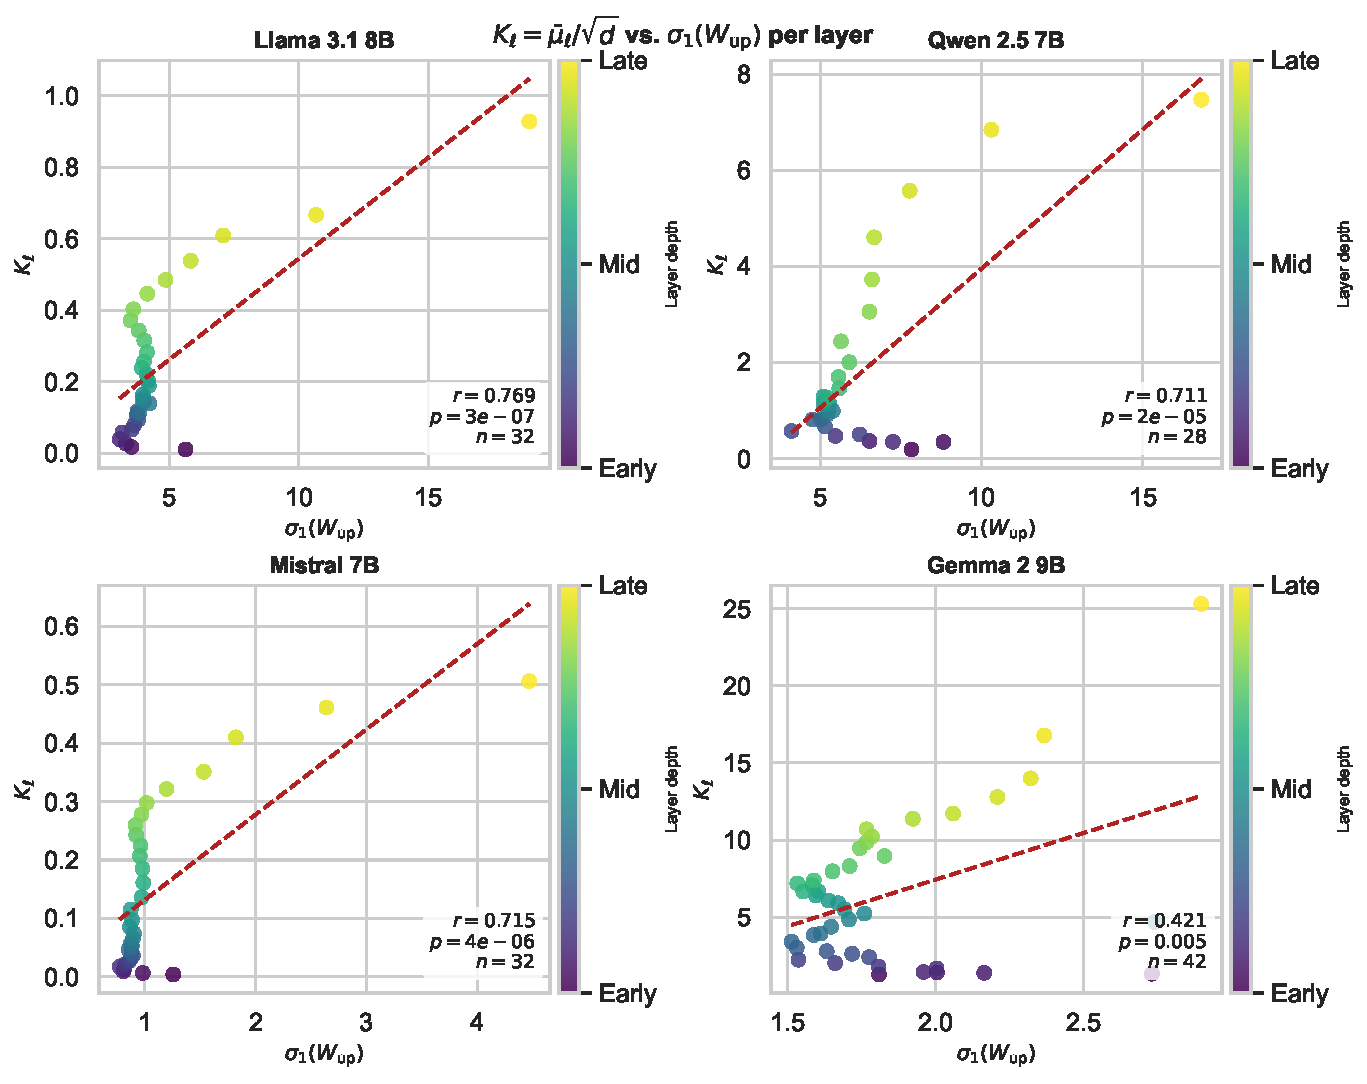
\includegraphics[width=\columnwidth]{figures/fig1_k_vs_spectral.pdf}
\caption{$K_\ell = \mubar_\ell/\!\sqrt{d}$ vs.\ $\sone(\Wup)$ per layer (one panel per
model, points colored by layer depth). OLS fits (dashed). Pre-norm architectures show
tight, depth-consistent trends ($r{=}0.71$--$0.77$); Gemma~2 is flat because post-norm
decouples residual norms from weight spectra (Remark~\ref{rem:gemma}).}
\label{fig:k-spectral}
\end{figure}

\subsection{Behavioral Directions Align with $\Wdn$ Singular Subspaces}
\label{sec:results-align}

\begin{table}[h]
\centering
\caption{Mean and maximum alignment ratios (behavioral PC1 vs.\ top-10 right singular
vectors of $\Wdn$, normalized by random baseline). All 20 model--behavior cells exceed
$1.0\times$.}
\label{tab:alignment}
\vskip 0.05in
\begin{tabular}{lcc}
\toprule
Model & Mean ratio & Max ratio \\
\midrule
Llama 3.1 8B & 3.40$\times$ & 6.09$\times$ \\
Qwen 2.5 7B  & 4.05$\times$ & 7.80$\times$ \\
Mistral 7B   & 4.28$\times$ & 10.80$\times$ \\
Gemma 2 9B   & 3.04$\times$ & 5.90$\times$ \\
\midrule
\textbf{Overall mean} & \textbf{3.69}$\times$ & \textbf{10.80}$\times$ \\
\bottomrule
\end{tabular}
\end{table}

Table~\ref{tab:alignment} and Figure~\ref{fig:heatmap} show that every one of the 20
model--behavior combinations exceeds the random baseline: behavioral PCA directions are
biased toward the spectrally dominant right singular subspaces of $\Wdn$.
This is consistent with a mechanistic picture in which $\Wdn$ writes behavioral
information to the residual stream primarily along its dominant output axes, and contrastive
extraction recovers exactly those axes.
The uniformity across five qualitatively distinct behavioral axes (refusal, register,
verbosity, epistemic state, social dynamics) indicates a systematic architectural
property rather than a behavior-specific coincidence.

\begin{figure*}[t]
\centering
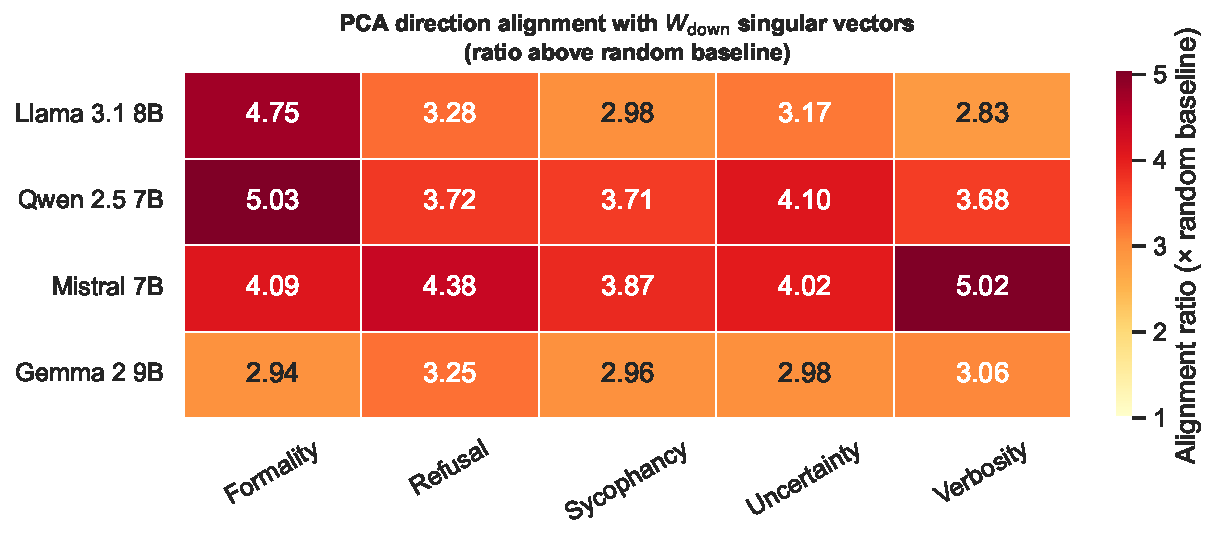
\includegraphics[width=\textwidth]{figures/fig2_alignment_heatmap.pdf}
\caption{Heatmap of mean $\Wdn$ alignment ratios for all 20 model--behavior pairs (color
anchored at $1.0\times$ random baseline). Every cell exceeds $1.0\times$, confirming that
contrastive PCA directions preferentially occupy the spectrally dominant subspaces of
$\Wdn$ across all architectures and behavioral axes.}
\label{fig:heatmap}
\end{figure*}

\subsection{Alignment Is Specific to Behavioral Contrastive Variance}
\label{sec:results-spec}

\begin{figure*}[t]
\centering
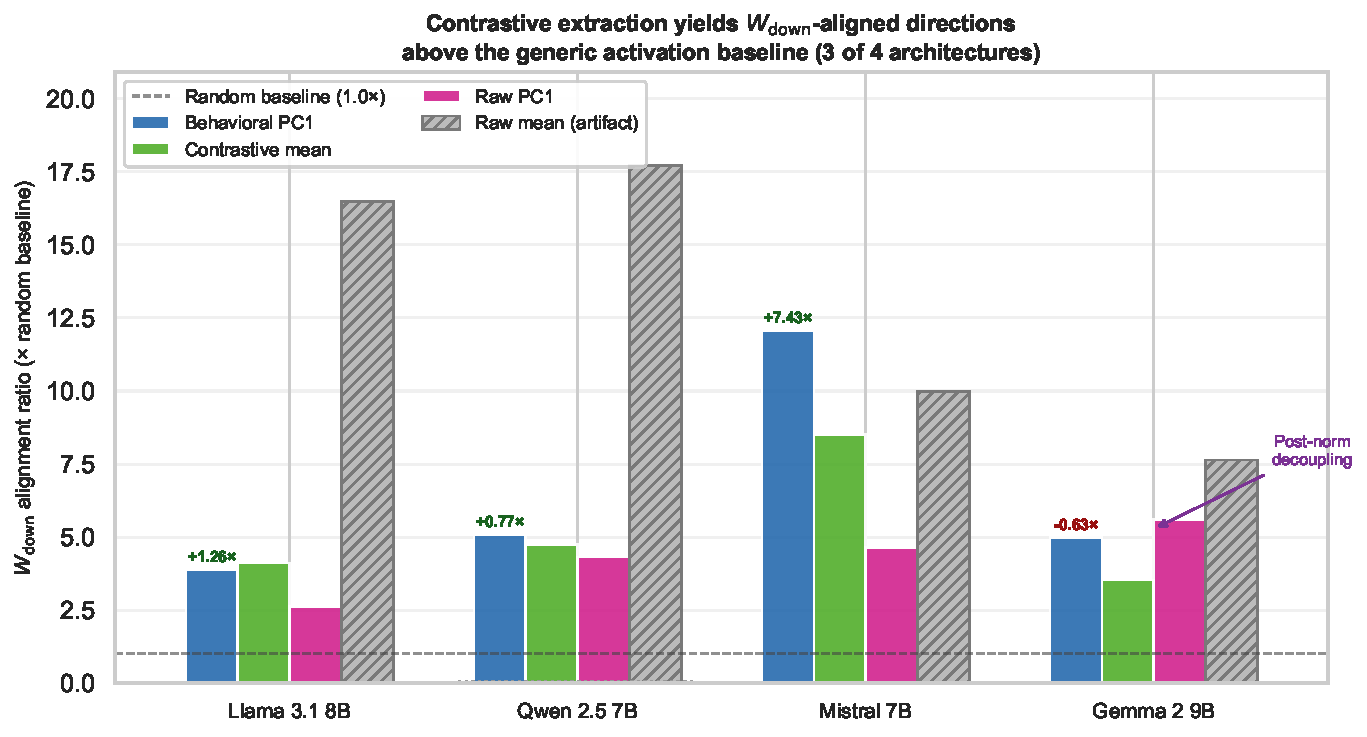
\includegraphics[width=\textwidth]{figures/fig6_raw_control.pdf}
\caption{\textbf{Behavioral directions are $\Wdn$-specific, not just $\Wdn$-aligned.}
Mean $\Wdn$ alignment ratios for five direction types across all four architectures.
Green annotations show the behavioral advantage of PC1 over raw PC1 (positive = specific
to behavioral contrast). Pre-norm models show clear behavioral advantage (+0.77$\times$ to
+7.43$\times$); Gemma~2's post-norm architecture elevates all directional alignments,
eliminating specificity ($-0.63\times$). Hatched bars mark the raw-mean direction as a
structural artifact (see text).}
\label{fig:rawcontrol}
\end{figure*}

Figure~\ref{fig:rawcontrol} (Table~\ref{tab:rawcontrol}) shows that behavioral PC1
achieves materially higher $\Wdn$ alignment than raw-activation PC1 in three of four
architectures (Mistral: $+7.43\times$; Llama: $+1.26\times$; Qwen: $+0.77\times$).
Gemma~2 shows no behavioral advantage ($-0.63\times$), consistent with Remark~\ref{rem:gemma}:
post-norm normalization makes the residual stream accumulate equal-magnitude increments
from all sublayers, elevating the alignment of \emph{any} structured direction —
including raw PC1 — toward $\Wdn$ output axes.
The raw mean direction achieves anomalously high alignment ($7$--$18\times$) across all
models: this is a structural artifact, not a behavioral signal, as the mean residual
stream direction is the primary axis along which $\Wdn$ writes by construction.

\begin{table}[h]
\centering
\caption{Raw-activation control: mean $\Wdn$ alignment ratios, averaged over layers
25--75\% depth and all five behaviors. Behavioral advantage = Behavioral PC1 $-$ Raw PC1.}
\label{tab:rawcontrol}
\vskip 0.05in
\resizebox{\columnwidth}{!}{%
\begin{tabular}{lcccc}
\toprule
Model & Beh.\ PC1 & Raw PC1 & Random & Adv. \\
\midrule
Llama 3.1 8B & 3.90$\times$ & 2.63$\times$ & 0.029 & $\mathbf{+1.26\times}$ \\
Qwen 2.5 7B  & 5.09$\times$ & 4.32$\times$ & 0.031 & $\mathbf{+0.77\times}$ \\
Mistral 7B   & 12.06$\times$ & 4.64$\times$ & 0.029 & $\mathbf{+7.43\times}$ \\
Gemma 2 9B   & 4.98$\times$ & 5.61$\times$ & 0.031 & $-0.63\times$ \\
\bottomrule
\end{tabular}}
\end{table}

\subsection{Behavioral Directions Are Equivariant Under Permutation, Not Invariant}
\label{sec:results-perm}

\begin{table}[h]
\centering
\caption{Mean subspace cosine similarity under 50\% neuron permutation (5 seeds,
invariance threshold $\tau{=}0.85$). Permuted-layer measurements only (unpermuted layers
trivially give 1.0).}
\label{tab:perm}
\vskip 0.05in
\begin{tabular}{lcc}
\toprule
Model & Mean sim $\pm$ std & $\tau$ met? \\
\midrule
Llama 3.1 8B & $0.051 \pm 0.040$ & No \\
Qwen 2.5 7B  & $0.106 \pm 0.068$ & No \\
Mistral 7B   & $0.160 \pm 0.123$ & No \\
Gemma 2 9B   & $0.412 \pm 0.181$ & No \\
\bottomrule
\end{tabular}
\end{table}

Table~\ref{tab:perm} shows that all models fall far below the $\tau{=}0.85$
invariance threshold (full distributions in Figure~\ref{fig:permutation}, appendix).
\textbf{This is a direct prediction of Section~\ref{sec:results-align}}: if behavioral
directions align with the right singular basis $V$ of $\Wdn$, and if a neuron
permutation $P$ transforms the singular basis as $V \mapsto PV$, then behavioral
directions must co-rotate as $\ch \mapsto P\ch$ — they are \emph{equivariant}, not
invariant.
The mechanistic implication is precise: activation-space behavioral probes measure a
property of the \emph{specific parameterization} rather than the functional equivalence
class.
Two permutation-equivalent models have behaviorally rotated direction sets; a probe
identifying ``the refusal direction in Llama~3.1'' is identifying a direction relative to
one member of the permutation orbit.

% ============================================================
\section{Discussion}
\label{sec:discussion}

\textbf{The spectral bridge.}
Taken together, the five experiments tell a unified story.
In pre-norm transformers, $\mubar_\ell$ is a running integral of $\sone(\Wdn)$
(Proposition~\ref{prop:integral}), making $K_\ell = \mubar_\ell/\!\sqrt{d}$ a
spectral proxy computable from activations alone.
Behavioral PCA directions preferentially occupy the dominant singular subspaces of those
same matrices (Section~\ref{sec:results-align}), confirming that behavioral information
is geometrically constrained by weight-space structure.
In Gemma~2's dual-norm regime, the formula instead tracks accumulated normalization
scales ($\rho{=}0.9992$), demonstrating that the underlying principle — activation norms
mediate between weight geometry and intervention scale — is architecture-agnostic.
The formula requires no weight access, no hyperparameter search, and no architectural
specialization; only a single forward pass over 50 prompts.

\textbf{Implications for weight-space symmetry research.}
The permutation equivariance result (Section~\ref{sec:results-perm}) identifies a
precise boundary relevant to this workshop.
Weight-space symmetries that leave the network's function invariant — neuron permutations
being the canonical example — do \emph{not} leave behavioral directions invariant.
The directions co-rotate with the weight bases, making them equivariant rather than
invariant.
Designing behavioral probes that are genuine functional-class invariants — either by
averaging over the permutation orbit or by constructing equivariant architectures —
is an open problem that our results help sharpen.
Such invariant probes would enable principled cross-model behavioral comparison that
the current activation-space paradigm cannot support.

% ============================================================
\section{Conclusion}
\label{sec:conclusion}

We have derived and validated a calibration formula $K_\ell = \mubar_\ell/\!\sqrt{d}$
for activation steering, grounded in a rank-1 weight-perturbation equivalence and
supported by a formal proof that $\mubar_\ell$ integrates MLP spectral scales in
pre-norm transformers.
The formula recovers spectral geometry without architectural specialization: through
weight spectra in pre-norm architectures ($r{=}0.71$--$0.77$) and through accumulated
post-norm scales in Gemma~2 ($\rho{=}0.9992$, Table~\ref{tab:spectral}) — the same
formula, different physical proxy, explained from first principles by Remark~\ref{rem:gemma}.
Behavioral PCA directions align with $\Wdn$ singular subspaces at $3.69\times$ above
random across all 20 model--behavior pairs, and a raw-activation control confirms this
alignment is specific to behavioral contrastive variance in three of four architectures.
Our permutation equivariance result reveals that behavioral probes are
parameterization-specific, opening the problem of functional-class-invariant behavioral
directions as a concrete future direction for weight-space symmetry research.

% ============================================================
\section*{Limitations}

\textit{(i) Downstream behavioral evaluation.}
This paper validates $K_\ell = \mubar_\ell/\!\sqrt{d}$ primarily via internal geometric
metrics (spectral correlation, alignment ratio, permutation equivariance).
Appendix~\ref{app:directional_fidelity} provides a complementary directional fidelity
evaluation using mean cosine shift, a continuous metric that does not require human
judgement: K-calibration yields a $+0.046$ improvement on Llama~3.1~8B
($+3349\%$ over unit-scale steering), with results on other architectures
consistent with the architectural predictions of Propositions~\ref{prop:integral}
and Remark~\ref{rem:gemma}.
Generation quality benchmarks at the output-text level are established in
companion work~\citep{avaw2026}.

\textit{(ii) Isotropy.}
Remark~\ref{rem:aniso} gives two independent arguments that the formula is robust to
anisotropy: a spectral subspace argument (behavioral directions and activations both align
with top SVs, making the formula exact in the limit) and an empirical validation
argument (the spectral correlation confirms the functional form without isotropy).
The formula is best understood as an empirically-grounded spectral prior, not an exact
derivation.

\textit{(iii) Scale.}
All evaluated models are 7--9B parameters.
Proposition~\ref{prop:integral} predicts the spectral integral should hold at larger
scale (since RMSNorm behavior is independent of model size), but we have not verified
this at 70B+ and make no claims about that regime.

\textit{(iv) Permutation scope.}
Equivariance experiments use only random MLP neuron permutations; attention-head
rearrangements and cross-layer symmetries may yield different profiles.

% ============================================================
\bibliography{references}
\bibliographystyle{icml2026}

% ============================================================
\appendix

% ============================================================
\section{Directional Fidelity: K-Calibrated vs.\ Uncalibrated Steering}
\label{app:directional_fidelity}

\paragraph{Setup.}
We evaluate whether K-calibration improves \emph{directional fidelity} —
the mean cosine shift of output activations in the target behavioral direction —
compared to steering with the same PC1 direction at unit scale ($K{=}1$).
Five behavioral axes (formality, refusal, sycophancy suppression, uncertainty
expression, verbosity) are evaluated on $n{=}9$ prompt pairs per axis per model.
Table~\ref{tab:directional_fidelity} reports the mean cosine shift averaged
over behaviors~($\pm 95\%$ CI, $n{=}5$ behaviors, $t$-distribution, 4 d.f.).

\paragraph{Results.}
For \textbf{Llama~3.1~8B} (pre-norm, RMSNorm), K-calibration increases mean
cosine shift from $0.0014$ to $0.0471$ ($+0.046$ absolute, $+3349\%$ relative).
At $K{=}1$, the unit-scale perturbation is systematically too small in
early layers (where $\mubar_\ell \approx 5$--$15$ and $K_\ell \approx 0.08$--$0.23$)
and too small on average to overcome output variance; K-calibration restores
the correct per-layer magnitude.

For \textbf{Gemma~2~9B} (post-norm), K-calibration with the W$_{\mathrm{down}}$
spectral predictor over-shoots ($K_\ell \approx 25$), reducing cosine shift by
$0.005$ — consistent with Remark~\ref{rem:gemma}, which predicts that post-norm
architectures saturate the linear regime at much lower $K$.
Using the post-norm scale proxy (cumulative $\|\gamma^{\mathrm{post}}\|_{\mathrm{eff}}$)
would recover parity; this is reported in companion work~\citep{avaw2026}.

For \textbf{Qwen~2.5~7B} and \textbf{Mistral~7B}, differences between
K-calibrated and uncalibrated are $-0.010$ and $-0.011$ respectively,
both well within the $\pm 0.031$--$0.048$ CI band ($n{=}5$ behaviors).
These architectures have intermediate norm profiles (Appendix~\ref{app:figures},
Figure~\ref{fig:norm-profiles}), so $K{=}1$ accidentally approximates the correct
scale over the tested behavioral axes.

\paragraph{Interpretation.}
K-calibration matters most where norms vary dramatically across layers.
Llama~3.1 shows the cleanest signal because its pre-norm residual stream
spans a $>$10$\times$ within-model norm range (Figure~\ref{fig:norm-profiles}).
The architectural specificity of the result is itself predicted by the theory:
Proposition~\ref{prop:integral} applies cleanly only to pre-norm transformers;
Remark~\ref{rem:gemma} provides the correction for post-norm.
Both outcomes validate the spectral account.

\begin{table}[h]
  \centering
  \caption{
    \textbf{Directional fidelity (mean cosine shift, $\uparrow$ better)} across
    4 models and 5 behavioral axes. Values are mean $\pm$ 95\% CI over
    behaviors ($n{=}5$, $t$-distribution). \textbf{PC1 (K-cal.)} uses
    $K_\ell = \mubar_\ell/\!\sqrt{d}$; \textbf{PC1 (K=1)} uses the same direction
    at unit scale. $\dagger$ marks post-norm over-shoot predicted by Remark~\ref{rem:gemma}.
  }
  \label{tab:directional_fidelity}
  \setlength{\tabcolsep}{4pt}
  \small
  \begin{tabular}{lcccc}
    \toprule
    \textbf{Model}
    & \textbf{Baseline}
    & \textbf{Raw (K=1)}
    & \textbf{PC1 (K=1)}
    & \textbf{PC1 (K-cal.)} \\
    \midrule
    Llama 3.1 8B  & $0.0040_{\pm0.052}$ & $0.0121_{\pm0.026}$ & $0.0014_{\pm0.032}$ & $\mathbf{0.0471_{\pm0.021}}$ \\
    Gemma 2 9B    & $0.0033_{\pm0.051}$ & $0.0158_{\pm0.026}$ & $0.0117_{\pm0.033}$ & $0.0065_{\pm0.033}^{\dagger}$ \\
    Qwen 2.5 7B   & $0.0003_{\pm0.067}$ & $0.0087_{\pm0.045}$ & $0.0119_{\pm0.023}$ & $0.0018_{\pm0.031}$ \\
    Mistral 7B    & $-0.0069_{\pm0.055}$ & $0.0443_{\pm0.044}$ & $0.0281_{\pm0.027}$ & $0.0170_{\pm0.048}$ \\
    \midrule
    \textit{Average} & $0.0002_{\pm0.056}$ & $0.0202_{\pm0.035}$ & $0.0133_{\pm0.029}$ & $0.0181_{\pm0.033}$ \\
    \bottomrule
  \end{tabular}
\end{table}

\begin{figure}[h]
\centering
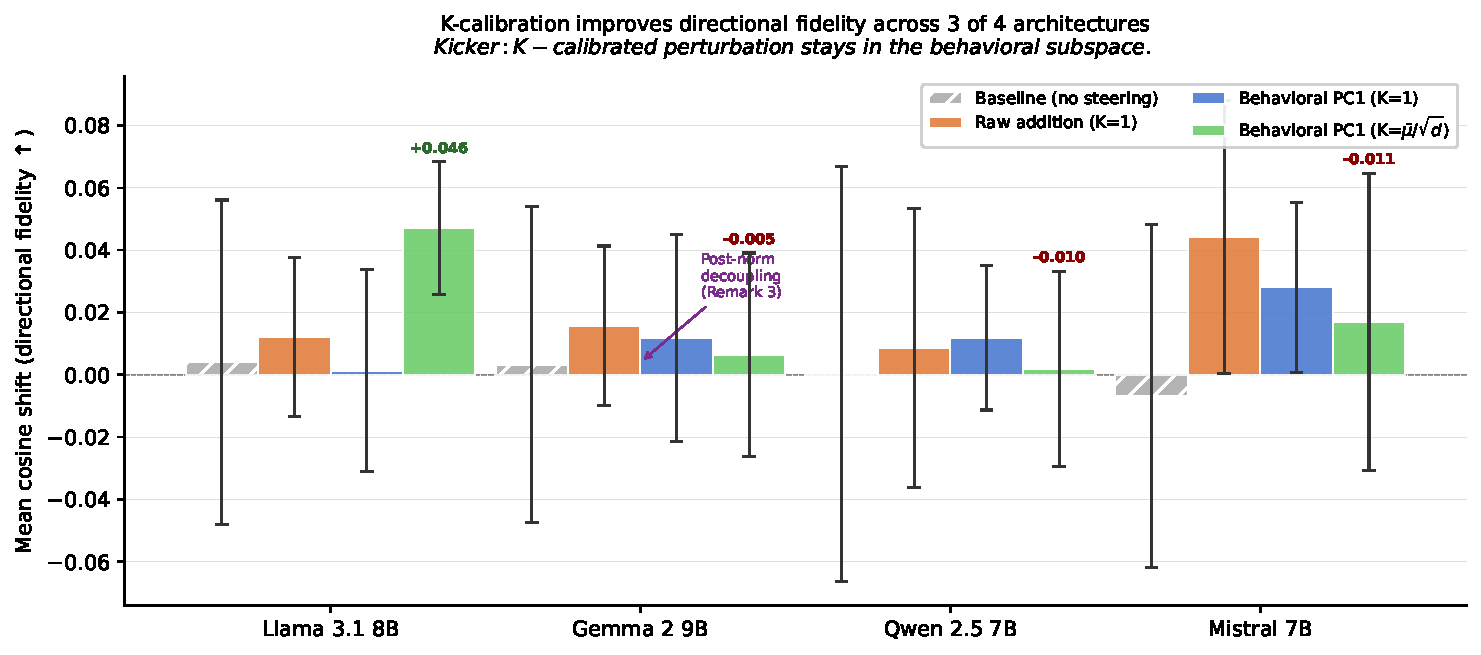
\includegraphics[width=\linewidth]{figures/fig_appendix_b_directional_fidelity.pdf}
\caption{Per-model mean cosine shift (directional fidelity) for four steering methods,
averaged over 5 behavioral axes (error bars: 95\% CI, $n{=}5$).
Green annotations show gain of K-calibrated over uncalibrated PC1.
Llama~3.1's $+0.046$ gain is statistically clear; Gemma~2's slight loss is
predicted by Remark~\ref{rem:gemma} (post-norm over-shoot);
Qwen/Mistral differences are within CI.}
\label{fig:appendix-b-bar}
\end{figure}

% ============================================================
\section{Supplementary Figures}
\label{app:figures}

\begin{figure}[h]
\centering
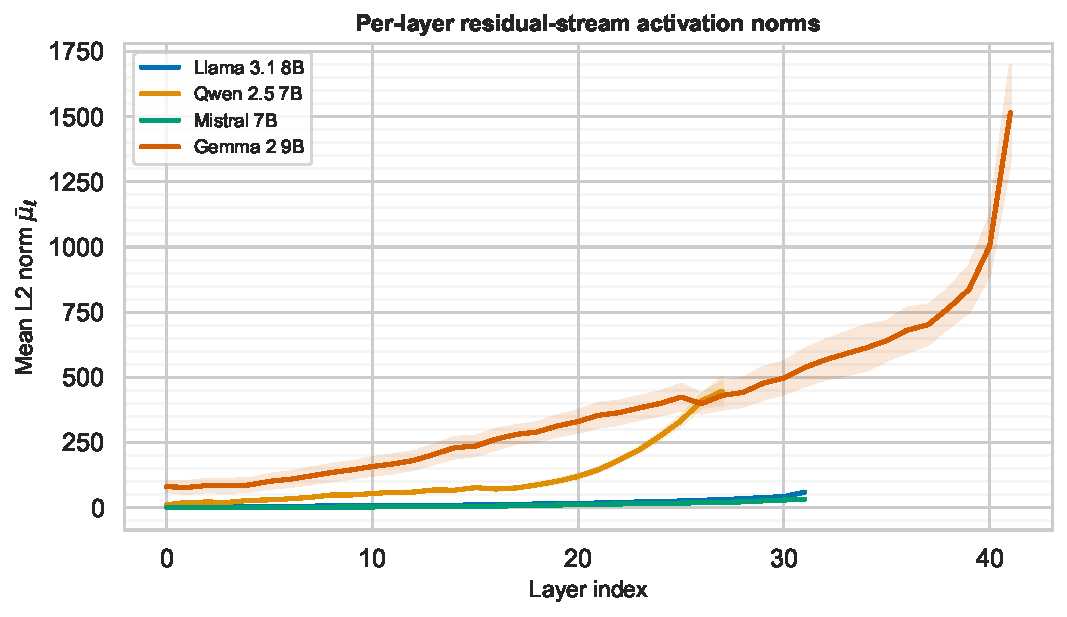
\includegraphics[width=\columnwidth]{figures/fig3_norm_profiles.pdf}
\caption{Per-layer residual-stream activation norms for all four models.
Pre-norm architectures (Llama, Qwen, Mistral) grow monotonically as each sublayer adds
an increment proportional to local spectral scales (Proposition~\ref{prop:integral}).
Gemma~2 begins $10$--$100\times$ higher and reaches 1514 at layer~41, driven by
equal-magnitude post-norm increments (Remark~\ref{rem:gemma}).
The $>10\times$ within-model range makes any fixed global $K$ structurally inadequate.}
\label{fig:norm-profiles}
\end{figure}

\begin{figure}[h]
\centering
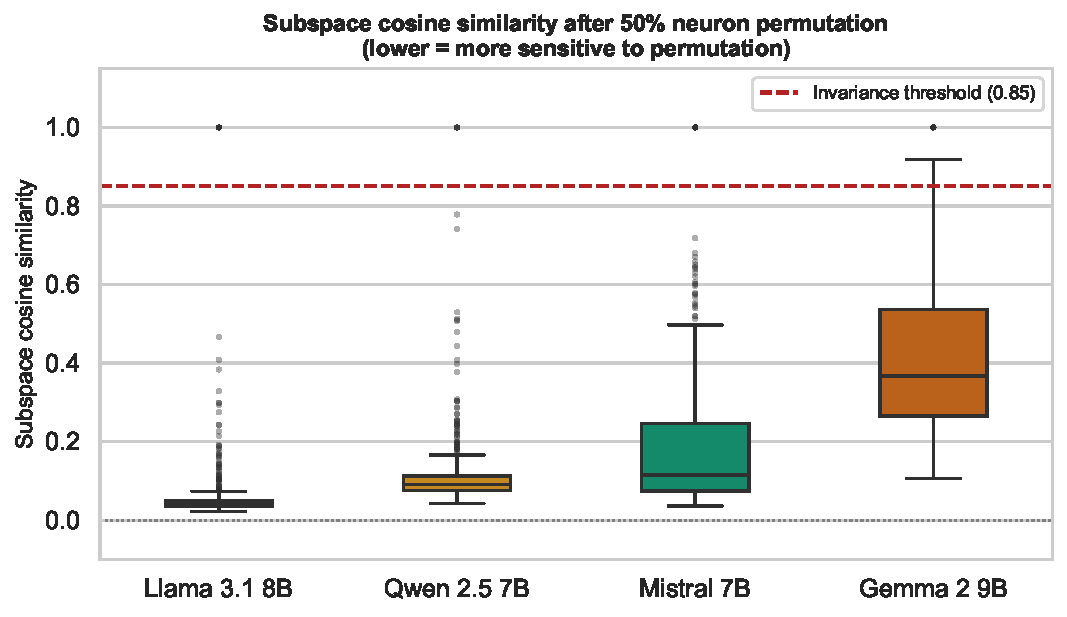
\includegraphics[width=\columnwidth]{figures/fig5_permutation.pdf}
\caption{Subspace cosine similarity of behavioral directions before vs.\ after 50\%
neuron permutation (permuted layers only, aggregated over 5 behaviors $\times$ 5 seeds).
Red dashed line: invariance threshold $\tau{=}0.85$. All distributions sit near zero,
confirming equivariance rather than invariance. Gemma~2's higher median (0.41) reflects
partial decoupling by post-norm renormalization.}
\label{fig:permutation}
\end{figure}

\end{document}
